\chapter{Resultados computacionales}
\label{resul_compu}

En este capítulo se presentan los resultados de los experimentos que se ejecutaron para ajustar algunos parámetros del algoritmo y para verificar el efecto de la aleatoriedad en el mismo.

Para ello se toma el grafo de 5 etapas y 13 nodos con valores fijos para sus respectivos \textit{bandits}, los cuales tiene la característica que, en cada etapa, uno de ellos es suficientemente mejor que los demás y hará que, seguramente, tal nodo forme parte  del vector de acciones seleccionadas al final de las 5 etapas. 

Los valores que se fijaron para la matriz de adyacencia y para los \textit{bandits} reales son los siguientes:

\renewcommand{\arraystretch}{0.5}
%\begin{equation}
A = 
$\begin{bmatrix}
%\hspace{2cm}

0, 1, 1,  1,  0,  0,  0,  0,  0,  0,  0,  0,  0\\
0, 0, 0,  0,  0,  1,  1,  1,  1,  0,  0,  0,  0\\
0, 0, 0,  0,  1,  1,  0,  1,  1,  0,  0,  0,  0\\
0, 0, 0,  0,  0,  1,  1,  0,  0,  0,  0,  0,  0\\
0, 0, 0,  0,  0,  0,  0,  0,  0,  1,  0,  1,  0\\
0, 0, 0,  0,  0,  0,  0,  0,  0,  0,  0,  1,  0\\
0, 0, 0,  0,  0,  0,  0,  0,  0,  0,  1,  1,  0\\
0, 0, 0,  0,  0,  0,  0,  0,  0,  0,  0,  1,  0\\
0, 0, 0,  0,  0,  0,  0,  0,  0,  0,  1,  0,  0\\
0, 0, 0,  0,  0,  0,  0,  0,  0,  0,  0,  0,  1\\
0, 0, 0,  0,  0,  0,  0,  0,  0,  0,  0,  0,  1\\
0, 0, 0,  0,  0,  0,  0,  0,  0,  0,  0,  0,  1\\
0, 0, 0,  0,  0,  0,  0,  0,  0,  0,  0,  0,  0
\end{bmatrix}$

%\end{equation}

%\begin{figure}
%	\centering
%	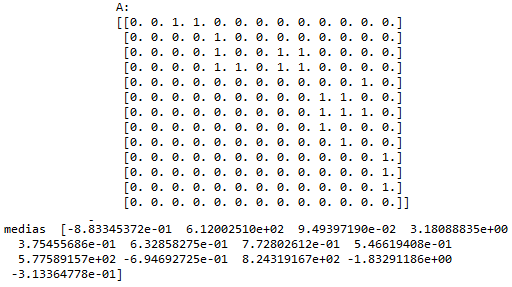
\includegraphics[scale=1]{MatrizAyBandits2}
%	\caption{Matriz y bandit generados}
%	\label{AyB}
%\end{figure}

$B$ = [2.29, 0.94, 193.06, -1.36, 190.22, -33.15, -0.42, -0.13, 2.46, 0.02, -0.81, 111.38, 1.38]

Es necesario tener en cuenta que aún se han dejando en forma aleatoria la selección inicial de los nodos y los valores distorsionados que se generan para los \textit{bandits} en cada iteración.

El grafo, con las aristas indicadas en la matriz de adyacencia y los valores de los \textit{bandits} del vector $B$, se aprecia en la figura \ref{Grafocaso1}
\begin{figure}[H]
	\centering
	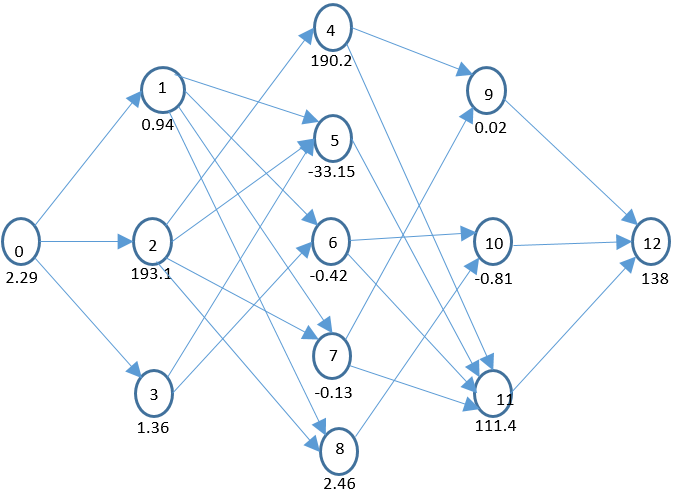
\includegraphics[scale=0.8]{Grafo5L.png}
	\caption{Grafo para las pruebas de parámetros}
	\label{Grafocaso1}
\end{figure}


\section{Parámetro Deltha puro}

Se retoman aquí las fórmulas con las que se consigue que el autómata aprenda y genere una matriz de probabilidades de transición entre nodos, para contextualizar al llamado \textbf{coeficiente de aprendizaje}. En la fórmula de probabilidades \ref{prob4} se observa que el exponente es una posición de un vector que se va actualizando de acuerdo al resultado de ganancia o pérdida de cada iteración, de la forma que se muestra en la fórmula \ref{exponente4}.
\begin{eqnarray}\label{prob4}
P(i \to j) = \frac{e^{v_j}}{\sum_k A_{i,k} e^{v_k}},
\end{eqnarray}
\begin{eqnarray}\label{exponente4}
v_j(\tau + 1) = v_j(\tau) \pm \delta,
\end{eqnarray}

\subsection{Prueba inicial}

Se realiza inicialmente una prueba con 9 valores para $\delta$ entre 0.1 y 0.9, sumando, en caso de ganancia y restando, en caso de pérdida, para motivar o desmotivar al autómata para que en el paso siguiente seleccione los nodos que reciben el refuerzo; la cantidad de iteraciones $T$ se varió entre 100 y 1000, con intervalos de 100. Las diferencias normalizadas que se encontraron entre la ganancia real y cada una de las ganancias que en promedio se obtuvieron se ven en la tabla \ref{tabla10}.

\begin{table}[H]
\small
\caption{Rangos de diferencia de ganancias con Deltha en décimas}
\begin{tabular}{crrrrrrrrrr}
\hline
\multicolumn{1}{l}{Deltha} & \multicolumn{10}{c}{Iteraciones} \\ \hline
\multicolumn{1}{l}{}       & \multicolumn{1}{c}{100} & \multicolumn{1}{c}{200} & \multicolumn{1}{c}{300} & \multicolumn{1}{c}{400} & \multicolumn{1}{c}{500} & \multicolumn{1}{c}{600} & \multicolumn{1}{c}{700} & \multicolumn{1}{c}{800} & \multicolumn{1}{c}{900} & \multicolumn{1}{c}{1000} \\ \hline
0,1                          & 0.715                    & 0.715                    & 0.715                    & 0.715                    & 0.715                    & 0.715                    & 0.715                    & 0.715                    & 0.715                    & 0.715                     \\ 
0,2                          & 0.695                    & 0.695                    & 0.695                    & 0.695                    & 0.695                    & 0.695                    & 0.695                    & 0.695                    & 0.695                    & 0.695                     \\ 
0,3                          & 0.676                    & 0.676                    & 0.676                    & 0.676                    & 0.676                    & 0.676                    & 0.676                    & 0.676                    & 0.676                    & 0.676                     \\ 
0,4                          & 0.656                    & 0.656                    & 0.656                    & 0.656                    & 0.656                    & 0.656                    & 0.656                    & 0.656                    & 0.656                    & 0.656                     \\ 
0,5                          & 0.637                    & 0.637                    & 0.637                    & 0.637                    & 0.637                    & 0.637                    & 0.637                    & 0.637                    & 0.637                    & 0.637                     \\ 
0,6                          & 0.618                    & 0.618                    & 0.618                    & 0.618                    & 0.618                    & 0.618                    & 0.618                    & 0.618                    & 0.618                    & 0.618                     \\ 
0,7                          & 0.598                    & 0.598                    & 0.598                    & 0.598                    & 0.598                    & 0.598                    & 0.598                    & 0.598                    & 0.598                    & 0.598                     \\ 
0,8                          & 0.579                    & 0.579                    & 0.579                    & 0.579                    & 0.579                    & 0.579                    & 0.579                    & 0.579                    & 0.579                    & 0.579                     \\ 
0,9                          & 0.559                    & 0.559                    & 0.559                    & 0.559                    & 0.559                    & 0.559                    & 0.559                    & 0.559                    & 0.559                    & 0.559                     \\ \hline
\end{tabular}
\label{tabla10}
\end{table}
Los rangos de diferencia superan el 50\%, independientemente de la cantidad de iteraciones que se ejecuten, por lo que se procede a experimentar con valores de $\deltha$ de órdenes diferentes. 

\subsection{Segunda prueba}

Se ejecuta la aplicación con valores de $\deltha$ en magnitudes de centésimas, milésimas y diezmilésimas y con los mismos 10 valores para la cantidad de iteraciones $T$, cuyos resultados se aprecian en la tabla \ref{tabla100_10000}.

\begin{table}[H]
\small

\caption{Rangos de diferencia de ganancias con Deltha en otras unidades}
\begin{tabular}{rrrrrrrrrrr} 
\multicolumn{1}{l}{Deltha} & \multicolumn{10}{c}{Iteraciones}      \\ \hline                                                                                                                                                                                              \\
\multicolumn{1}{l}{}       & 100                  & 200                  & 300                  & 400                  & 500                  & 600                  & 700                  & 800                  & 900                  & 1000                 \\
0.01                       & 0.697                & 0.697                & 0.671                & 0.695                & 0.675                & 0.677                & 0.661                & 0.694                & 0.654                & 0.692                \\
0.02                       & 0.707                & 0.686                & 0.628                & 0.583                & 0.565                & 0.605                & 0.661                & 0.751                & 0.760                & 0.809                \\
0.03                       & 0.615                & 0.698                & 0.763                & 0.744                & 0.742                & 0.734                & 0.777                & 0.512                & 0.813                & 0.819                \\
0.04                       & 0.646                & 0.651                & 0.533                & 0.783                & 0.812                & 0.800                & 0.505                & 0.495                & 0.815                & 0.820                \\
0.05                       & 0.816                & 0.720                & 0.780                & 0.795                & 0.504                & 0.484                & 0.483                & 0.798                & 0.817                & 0.492                \\
0.06                       & 0.607                & 0.475                & 0.806                & 0.555                & 0.809                & 0.537                & 0.459                & 0.817                & 0.819                & 0.476                \\
0.07                       & 0.725                & 0.764                & 0.774                & 0.810                & 0.824                & 0.514                & 0.824                & 0.831                & 0.837                & 0.822                \\
0.08                       & 0.654                & 0.806                & 0.450                & 0.472                & 0.492                & 0.476                & 0.490                & 0.421                & 0.471                & 0.466                \\
0.09                       & 0.756                & 0.765                & 0.502                & 0.604                & 0.486                & 0.820                & 0.780                & 0.775                & 0.827                & 0.835                \\ \hline
\multicolumn{1}{l}{}       & \multicolumn{1}{l}{} & \multicolumn{1}{l}{} & \multicolumn{1}{l}{} & \multicolumn{1}{l}{} & \multicolumn{1}{l}{} & \multicolumn{1}{l}{} & \multicolumn{1}{l}{} & \multicolumn{1}{l}{} & \multicolumn{1}{l}{} & \multicolumn{1}{l}{} \\
\multicolumn{1}{l}{Deltha} & \multicolumn{10}{c}{Iteraciones}   \\ \hline                                                                                                                                                                                                   \\
\multicolumn{1}{l}{}       & 100                  & 200                  & 300                  & 400                  & 500                  & 600                  & 700                  & 800                  & 900                  & 1000                 \\
0.001                      & 0.690                & 0.699                & 0.705                & 0.713                & 0.705                & 0.704                & 0.708                & 0.727                & 0.713                & 0.698                \\
0.002                      & 0.702                & 0.710                & 0.706                & 0.715                & 0.716                & 0.696                & 0.682                & 0.680                & 0.696                & 0.714                \\
0.003                      & 0.647                & 0.719                & 0.682                & 0.692                & 0.699                & 0.700                & 0.709                & 0.691                & 0.687                & 0.659                \\
0.004                      & 0.711                & 0.721                & 0.697                & 0.694                & 0.688                & 0.687                & 0.671                & 0.691                & 0.681                & 0.693                \\
0.005                      & 0.763                & 0.691                & 0.710                & 0.682                & 0.688                & 0.686                & 0.667                & 0.664                & 0.684                & 0.689                \\
0.006                      & 0.692                & 0.726                & 0.693                & 0.692                & 0.716                & 0.689                & 0.654                & 0.680                & 0.647                & 0.605                \\
0.007                      & 0.730                & 0.695                & 0.696                & 0.680                & 0.680                & 0.656                & 0.674                & 0.626                & 0.706                & 0.656                \\
0.008                      & 0.728                & 0.651                & 0.708                & 0.669                & 0.668                & 0.686                & 0.681                & 0.710                & 0.692                & 0.665                \\
0.009                      & 0.707                & 0.695                & 0.644                & 0.691                & 0.640                & 0.717                & 0.714                & 0.614                & 0.703                & 0.692                \\ \hline
\multicolumn{1}{l}{}       & \multicolumn{1}{l}{} & \multicolumn{1}{l}{} & \multicolumn{1}{l}{} & \multicolumn{1}{l}{} & \multicolumn{1}{l}{} & \multicolumn{1}{l}{} & \multicolumn{1}{l}{} & \multicolumn{1}{l}{} & \multicolumn{1}{l}{} & \multicolumn{1}{l}{} \\
\multicolumn{1}{l}{Deltha} & \multicolumn{10}{c}{Iteraciones}    \\ \hline                                                                                                                                                                                                  \\
\multicolumn{1}{l}{}       & 100                  & 200                  & 300                  & 400                  & 500                  & 600                  & 700                  & 800                  & 900                  & 1000                 \\
0.0001                     & 0.708                & 0.689                & 0.728                & 0.718                & 0.693                & 0.709                & 0.700                & 0.694                & 0.709                & 0.699                \\
0.0002                     & 0.684                & 0.697                & 0.718                & 0.696                & 0.710                & 0.734                & 0.700                & 0.706                & 0.708                & 0.699                \\
0.0003                     & 0.718                & 0.683                & 0.693                & 0.699                & 0.706                & 0.715                & 0.699                & 0.707                & 0.715                & 0.696                \\
0.0004                     & 0.748                & 0.717                & 0.704                & 0.707                & 0.710                & 0.745                & 0.705                & 0.705                & 0.707                & 0.713                \\
0.0005                     & 0.686                & 0.692                & 0.705                & 0.733                & 0.700                & 0.706                & 0.709                & 0.691                & 0.704                & 0.717                \\
0.0006                     & 0.649                & 0.742                & 0.703                & 0.711                & 0.699                & 0.685                & 0.717                & 0.706                & 0.707                & 0.706                \\
0.0007                     & 0.752                & 0.723                & 0.733                & 0.706                & 0.700                & 0.701                & 0.688                & 0.709                & 0.697                & 0.722                \\
0.0008                     & 0.682                & 0.725                & 0.704                & 0.706                & 0.720                & 0.690                & 0.700                & 0.712                & 0.705                & 0.709                \\
0.0009                     & 0.718                & 0.680                & 0.708                & 0.691                & 0.694                & 0.702                & 0.702                & 0.714                & 0.688                & 0.698          \\ \hline       
\end{tabular}
\label{tabla100_10000}
\end{table}

Aquí se puede apreciar que, a pesar de disminuir notablemente los valores de $deltha$, se siguen obteniendo valores muy altos para la diferencia de las ganancias, con errores superiores al 40\%. Los promedios de estas diferencias se presentan en la tabla \ref{delthas_0000}

\begin{table}[H]
\centering
%\small
\caption{Promedios de los resultados variando décimas en Deltha}
\begin{tabular}{llll} \\ \hline  
\multicolumn{4}{c}{\textbf{PROMEDIOS DE ERROR EN GANANCIAS}}                                                  \\ \hline  
\textbf{Décimas}          & \textbf{Centésimas}       & \textbf{Milésimas}        & \textbf{Diezmilésimas}    \\ \hline  
\multicolumn{1}{r}{0.637} & \multicolumn{1}{r}{0.675} & \multicolumn{1}{r}{0.690} & \multicolumn{1}{r}{0.706} \\ \hline  
\end{tabular}
\label{delthas_0000}
\end{table}

Con estos resultados, se formulan experimentos con una mayor variación para $deltha$ y para la cantidad de Iteraciones $T$, que permita un análisis estadístico de la influencia de estas dos variables en los resultados esperados.

\subsection{Experimentos}

\subsubsection{Variable dependiente}

Se define como variable dependiente para este conjunto de experimentos a la diferencia entre la ganancia máxima y la ganancia obtenida en la ejecución. Para estimar el error que se está generando a partir de esta diferencia, se normaliza esta última dividiéndola en el valor de la ganancia máxima, de forma que se obtengan valores entre cero y uno.

\subsubsection{Variables independientes}
Los experimentos se diseñan teniendo en cuenta que las variables independientes corresponden a: 
\begin{itemize}
    \item Factor de aprendizaje $\delta$
    \item Número de iteraciones
\end{itemize}

\subsubsection{Validez}
Para el control o validez interna se ha de comprobar que las variables, aquí definidas como independientes, son las que realmente influyen en las dependientes, y no factores externos como la aleatoriedad. Se toman, entonces, los resultados de 100 experimentos con cada uno de los valores de control sobre las variables independientes.

\subsubsection{Técnica}
La técnica que se usa en este experimento es la simulación. Es un instrumento objetivo, confiable y válido. La validez es alta, puesto que el computador siempre tratará los valores de la misma manera; se espera que con un mismo valor de variables independientes se obtengan resultados similares en las variables dependientes.

\subsubsection{Herramientas}
Se realizan los cálculos de medias, varianzas y de análisis de varianza (ANOVA) que permitan concluir la forma en que cada variable independiente influye en la dependiente.

\subsubsection{Experimento uno}

Se diseña un experimento con las las variables independientes: T y $\delta$, correspondientes a la cantidad de iteraciones y a la variable que ha de incentivar la selección o no de un nodo, con el aumento o disminución de probabilidad de ser preferido en las siguientes iteraciones y, por supuesto, en el camino óptimo, como se ve en la ecuación \ref{delta}, ya explicada en el modelo de la solución; la variable dependiente corresponde a la diferencia normalizada de las ganancias.
\begin{eqnarray}\label{delta}
v_j(\tau + 1) = v_j(\tau) \pm \delta,
\end{eqnarray}

%Se adiciona a la aplicación una variable que mide el porcentaje de veces que el vector final corresponde al esperado, la cual permite corroborar que las soluciones con diferencias de ganancia cercanas a cero, ofrecen, en una cantidad cercana al 100\%, el vector solución que se espera y que la convergencia de la ganancia obtenida, sí se está dando hacia la ganancia óptima.

Se usan valores para T de 100, 1000, 10000 y 100000 iteraciones y valores de $\delta$ de $10^{2}$, $10^{1}$, $10^{0}$, $10^{-1}$, $10^{-2}$, $10^{-3}$ y $10^{-4}$. Este experimento se ejecuta varias veces, encontrando diferentes valores en sus resultados para los mismo valores de T y de $\delta$, lo que se explica por la influencia de la aleatoriedad en estos resultados y se corrobora con el valor del estadístico de prueba F y el valor de P de las tablas ANOVA. Las gráficas correspondientes a tres ejecuciones de este experimento y los resultados del ANOVA correspondiente, se presentan en la tabla \ref{exp1}.
\begin{table}[H]
\caption{Experimento uno}
\centering
\begin{tabular}[c]{llll}
\multicolumn{1}{p{2.9cm}}{\textbf{GRÁFICA PARA $\delta$}} & \multicolumn{1}{p{2.9cm}}{\textbf{GRÁFICA PARA $T$}} & \multicolumn{1}{p{2.9cm}}{\textbf{GRÁFICA PARA $T$ y $\delta$}} & \multicolumn{1}{p{2.9cm}}{\textbf{ANOVA}}  \\ \hline
\multicolumn{1}{|l|}{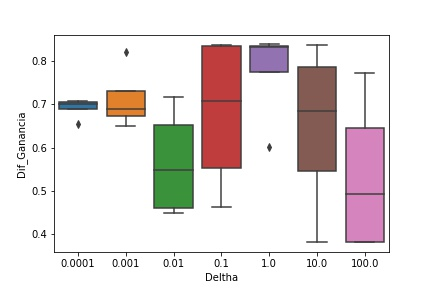
\includegraphics[align=t, width=33mm]{cajasDeltha_exp11.jpg}}    & \multicolumn{1}{l|}{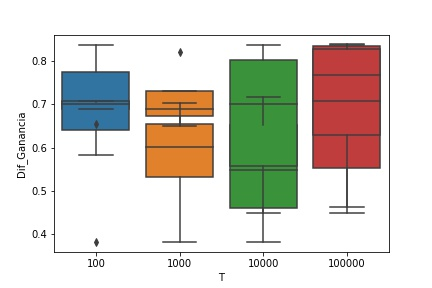
\includegraphics[align=t, width=33mm]{cajasT1_exp11.jpg} } & \multicolumn{1}{l|}{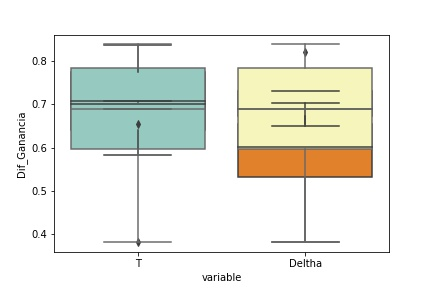
\includegraphics[align=t, width=33mm]{cajasT_Deltha_exp11.jpg} } &
\multicolumn{1}{p{3cm}|}{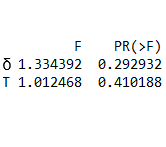
\includegraphics[align=t, width=30mm]{Anova11.png}}     \\ \hline
\multicolumn{1}{|l|}{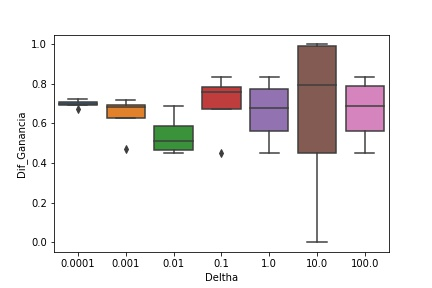
\includegraphics[align=t, width=33mm]{cajasDeltha_exp12.jpg}}    & \multicolumn{1}{l|}{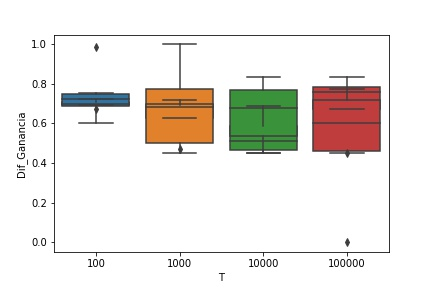
\includegraphics[align=t, width=33mm]{cajasT1_exp12.jpg} } & \multicolumn{1}{l|}{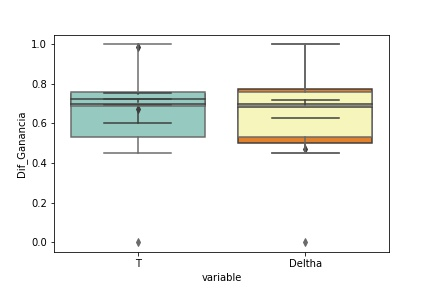
\includegraphics[align=t, width=33mm]{cajasT_Deltha_exp12.jpg} } & \multicolumn{1}{p{3cm}|}{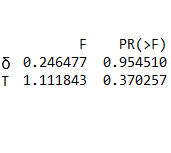
\includegraphics[align=t, width=30mm]{Anova12.png}} \\ \hline
\multicolumn{1}{|l|}{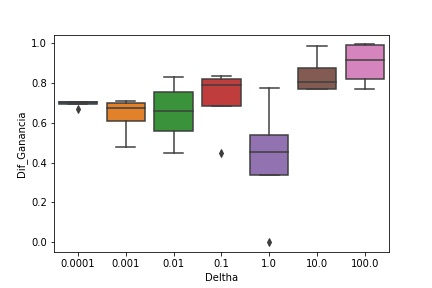
\includegraphics[align=t, width=33mm]{cajasDeltha_exp13.jpg}}    & \multicolumn{1}{l|}{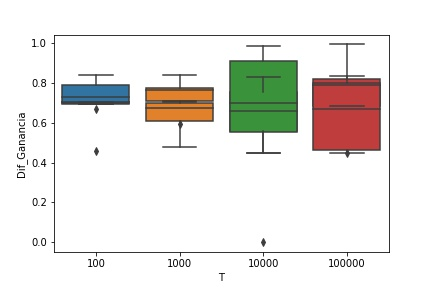
\includegraphics[align=t, width=33mm]{cajasT1_exp13.jpg} } & \multicolumn{1}{l|}{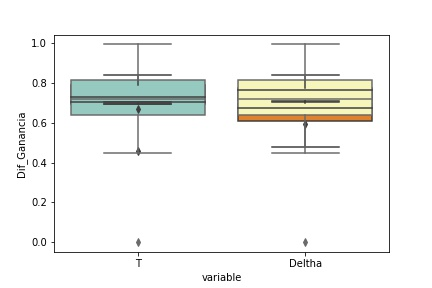
\includegraphics[align=t, width=33mm]{cajasT_Deltha_exp13.jpg} } & \multicolumn{1}{p{3cm}|}{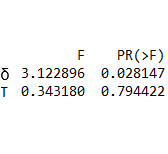
\includegraphics[align=t, width=30mm]{Anova13.png}} \\ \hline
\end{tabular}
\label{exp1}
\end{table}

En las tres filas de la tabla \ref{exp1} se notan cambios en las medias y las varianzas obtenidos de una ejecución a otra, y en las tablas ANOVA se puede verificar que la probabilidad $PR(>F)$ se mantuvo, en casi todos los caso, en valores superiores a 0.05, pero en el tercero, para la variable $Deltha$ sí se obtuvo un valor menor de 0.05 en dicha columna. Estos resultados no nos permiten concluir que las variables independientes tengan un alto grado de significancia sobre la variable dependiente; además, se esperaría que, en general, el estadístico de prueba $F$ tuviera siempre un valor distante de la unidad y no es así. 

Además estas gráficas muestran que, independientemente de la cantidad de iteraciones que se hagan (variable T, eje horizontal), se obtienen resultados muy altos para la diferencia normalizada de ganancias, con medias que llegan a estar por encima del 70\%. Coincide en las tres ocasiones que la varianza en las cajas para el menor valor de T es la más pequeña; esto se debe a que en estos casos, y especialmente cuando se tienen valores grandes para $\delta$, el algoritmo tiende a aprender una de las primeras respuestas que, aleatoriamente, debió validar y se queda con ella convergiendo rápidamente a cualquier respuesta que no es necesariamente la óptima. Se procede entonces a verificar lo que sucede con valores grandes para T y pequeños para $\delta$.

Se quiere observar si algunos de los valor de $T$ y de $delta$ que en la gráfica muestran mejores resultados, influyen efectivamente en la optimización de la diferencia entre ganancias.

\subsubsection{Experimento dos}

%Se diseña un experimento con las mismas dos variables independientes: T y $\delta$, y la misma variable dependiente corresponde a la diferencia normalizada de las ganancias que debe corresponder con los resultados del porcentaje de veces que el vector final corresponde al esperado.

Se usan, en esta ocasión, valores para $T$ de 100000 y 100001 (es decir, casi la misma cantidad) y valores de $delta$ de $10^{-3}$ y $10^{-4}$. Este experimento se ejecuta varias veces, encontrando diferentes valores en sus resultados para los mismos valores de $T$ y de $\delta$, lo que se explica como una alta influencia de la aleatoriedad. Tres resultados con los mismos valores de la variables independientes se muestran en la figura \ref{exp2}

\begin{table}[H]
\caption{Experimento dos}
\centering
\begin{tabular}[c]{llll}
\multicolumn{1}{p{2.9cm}}{\textbf{GRÁFICA PARA $\delta$}} & \multicolumn{1}{p{2.9cm}}{\textbf{GRÁFICA PARA $T$}} & \multicolumn{1}{p{2.9cm}}{\textbf{GRÁFICA PARA $T$ y $\delta$}} & \multicolumn{1}{p{2.9cm}}{\textbf{ANOVA}}  \\ \hline
\multicolumn{1}{|l|}{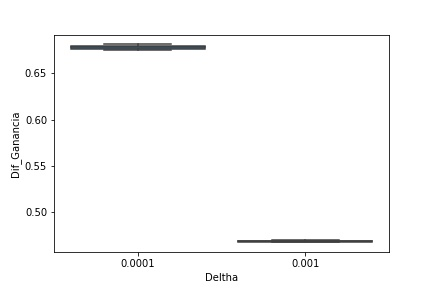
\includegraphics[align=t, width=33mm]{cajasDeltha_exp21.jpg}}    & \multicolumn{1}{l|}{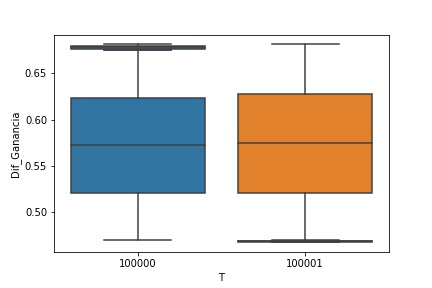
\includegraphics[align=t, width=33mm]{cajasT1_exp21.jpg} } & \multicolumn{1}{l|}{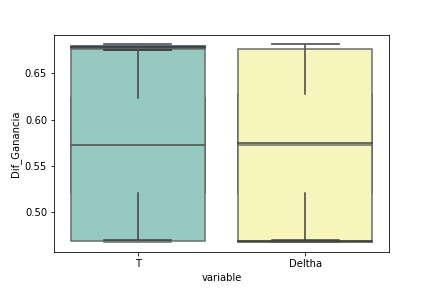
\includegraphics[align=t, width=33mm]{cajasT_Deltha_exp21.jpg} } &
\multicolumn{1}{p{3cm}|}{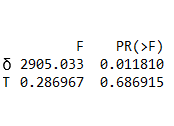
\includegraphics[align=t, width=30mm]{Anova21.png}}     \\ \hline
\multicolumn{1}{|l|}{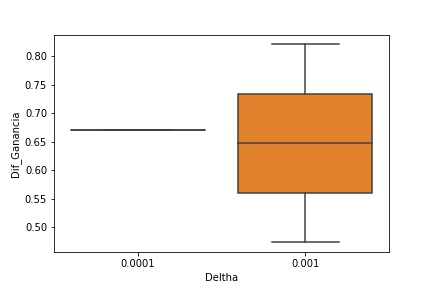
\includegraphics[align=t, width=33mm]{cajasDeltha_exp22.jpg}}    & \multicolumn{1}{l|}{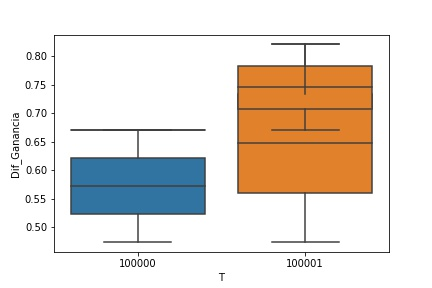
\includegraphics[align=t, width=33mm]{cajasT1_exp22.jpg} } & \multicolumn{1}{l|}{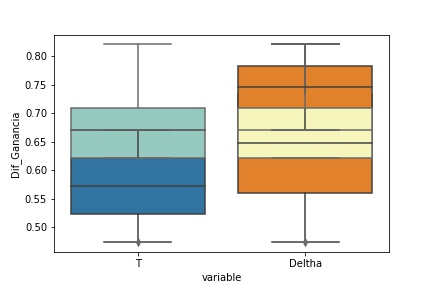
\includegraphics[align=t, width=33mm]{cajasT_Deltha_exp22.jpg} } & \multicolumn{1}{p{3cm}|}{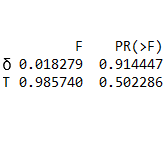
\includegraphics[align=t, width=30mm]{Anova22.png}} \\ \hline
\multicolumn{1}{|l|}{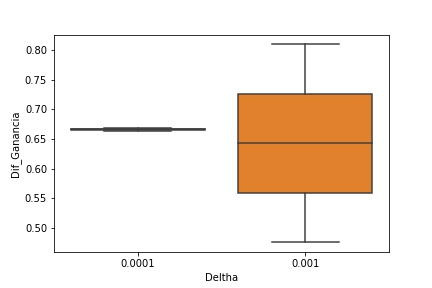
\includegraphics[align=t, width=33mm]{cajasDeltha_exp23.jpg}}    & \multicolumn{1}{l|}{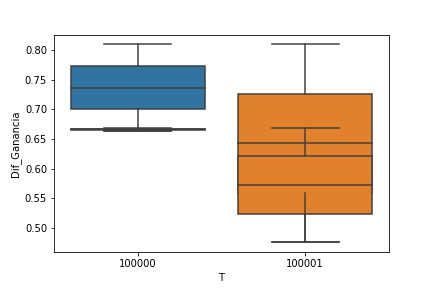
\includegraphics[align=t, width=33mm]{cajasT1_exp23.jpg} } & \multicolumn{1}{l|}{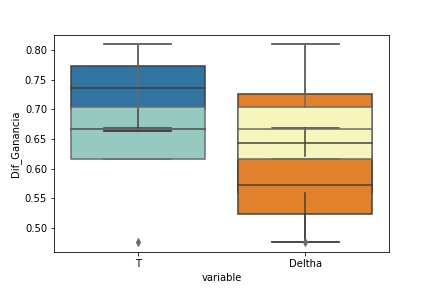
\includegraphics[align=t, width=33mm]{cajasT_Deltha_exp23.jpg} } & \multicolumn{1}{p{3cm}|}{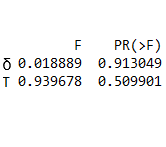
\includegraphics[align=t, width=30mm]{Anova23.png}} \\ \hline
\end{tabular}
\label{exp2}
\end{table}

Los resultados de las tablas ANOVA en la ejecución de la fila $1$ de la tabla \ref{exp2} presentan un valor para el estadístico de prueba $F$ mucho mayor que 1 y el valor de la probabilidad $PR(>F)$ menor a 0.05, para la variable $\delta$, lo que indicaría que esta variable independiente influye notoriamente en la variable dependiente; pero en las dos ejecuciones que se muestran al final de la tabla, no se mantuvo este resultado para $\delta$, obteniendo valores en $PR(>F)$ superiores a 0.05; así mismo para la variable $T$. Estos resultados no nos permiten, nuevamente, concluir que las variables independientes tengan un alto grado de significancia sobre la variable dependiente.

Se decide, entonces trabajar con una variable $\delta$ dependiente de la magnitud de la ganancia o pérdida que se reciba al final de cada ruta probada, como se explica en el siguiente experimento.

\section{Parámetro Gamma}

Se procede a experimentar con $delta$ autoajustable, que depende del valor de la ganancia que recibe la ruta probada, de forma que, inclusive, el signo se ajustará cuando hayan pérdidas, sin hacerse necesario decidir entre suma y resta. Se involucra una nueva variable Gamma ($\gamma$) a la que se le variarán sus valores y de la que se obtiene $\delta$ para la ecuación \ref{exponente5}, al multiplicar $\gamma$ por la ganancia o recompensa recibida al final del camino.
\begin{eqnarray}\label{exponente5}
v_j(\tau + 1) = v_j(\tau) + \delta,
\end{eqnarray}

\subsection{Primer caso de estudio}

Inicialmente se realizó una prueba para establecer el porcentaje de ejecuciones en que el algoritmo realmente converge, ejecutando varias veces el algoritmo con el grafo ya fijo. En esta, se ha encontrado una tendencia a que solo en 7 de cada 10 ocasiones se logra la convergencia hacia el valor real. Las gráficas de la figura \ref{Ejecuta10} corresponden a 10 corridas del algoritmo de probabilidades aprendidas con 1000 iteraciones, un $\delta$ de aprendizaje que se obtuvo de multiplicar $\gamma = 0.0003$ por el valor de la ganancia o recompensa de la ruta utilizada.

\begin{figure} 
    \centering
    \begin{subfigure}[b]{0.38\textwidth}
        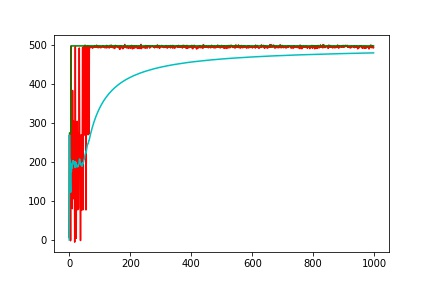
\includegraphics[width=\textwidth]{grafi1.jpg}
        %\caption{A gull}
        \label{fig:gull}
    \end{subfigure}
    \vspace{0.5 mm}
    ~ %add desired spacing between images, e. g. ~, \quad, \qquad, \hfill etc. 
      %(or a blank line to force the subfigure onto a new line)
    \begin{subfigure}[b]{0.38\textwidth}
        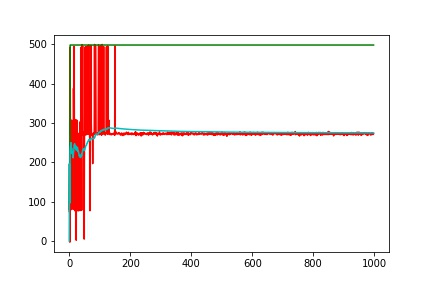
\includegraphics[width=\textwidth]{grafi2.jpg}
        %\caption{A tiger}
        \label{fig:tiger}
    \end{subfigure}
    ~ %add desired spacing between images, e. g. ~, \quad, \qquad, \hfill etc. 
    %(or a blank line to force the subfigure onto a new line)
    \begin{subfigure}[b]{0.38\textwidth}
        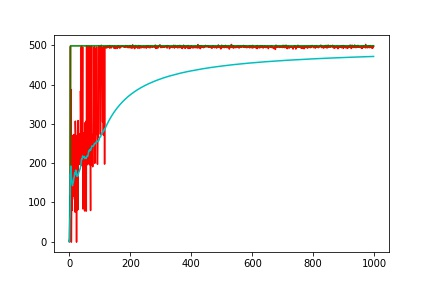
\includegraphics[width=\textwidth]{grafi3.jpg}
        %\caption{A mouse}
        \label{fig:mouse}
    \end{subfigure}
    \begin{subfigure}[b]{0.38\textwidth}
        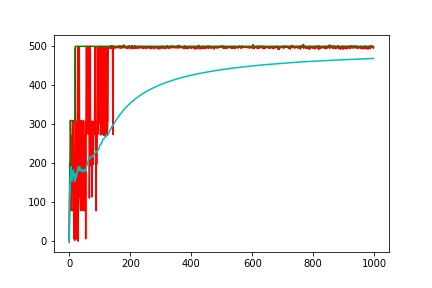
\includegraphics[width=\textwidth]{grafi4.jpg}
        %\caption{A tiger}
        \label{fig:tiger}
    \end{subfigure}
        \begin{subfigure}[b]{0.38\textwidth}
        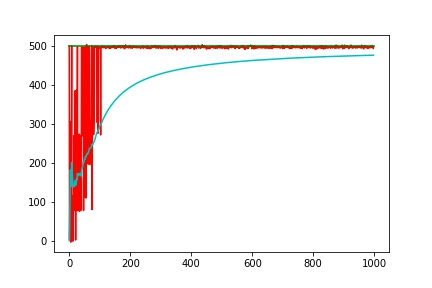
\includegraphics[width=\textwidth]{grafi5.jpg}
        %\caption{A gull}
        \label{fig:gull}
    \end{subfigure}
    ~ %add desired spacing between images, e. g. ~, \quad, \qquad, \hfill etc. 
      %(or a blank line to force the subfigure onto a new line)
    \begin{subfigure}[b]{0.38\textwidth}
        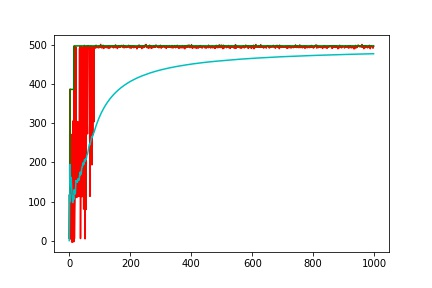
\includegraphics[width=\textwidth]{grafi6.jpg}
        %\caption{A tiger}
        \label{fig:tiger}
    \end{subfigure}
    ~ %add desired spacing between images, e. g. ~, \quad, \qquad, \hfill etc. 
    %(or a blank line to force the subfigure onto a new line)
    \begin{subfigure}[b]{0.38\textwidth}
        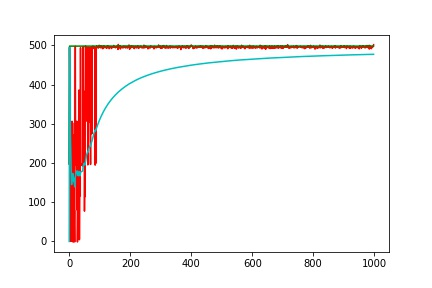
\includegraphics[width=\textwidth]{grafi7.jpg}
        %\caption{A mouse}
        \label{fig:mouse}
    \end{subfigure}
    \begin{subfigure}[b]{0.38\textwidth}
        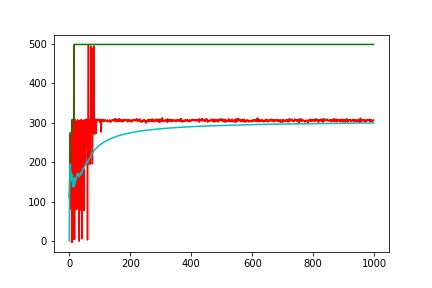
\includegraphics[width=\textwidth]{grafi8.jpg}
        %\caption{A tiger}
        \label{fig:tiger}
    \end{subfigure}
    \begin{subfigure}[b]{0.38\textwidth}
        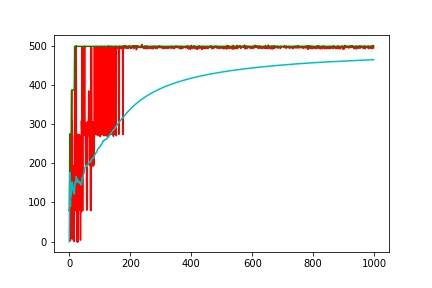
\includegraphics[width=\textwidth]{grafi9.jpg}
        %\caption{A mouse}
        \label{fig:mouse}
    \end{subfigure}
    \begin{subfigure}[b]{0.38\textwidth}
        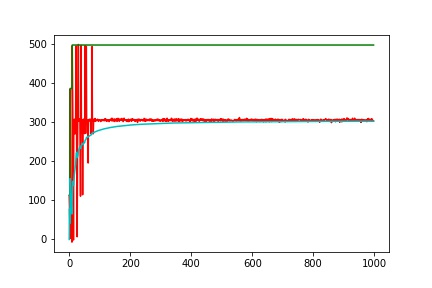
\includegraphics[width=\textwidth]{grafi10.jpg}
        %\caption{A tiger}
        \label{fig:tiger}
    \end{subfigure}    
    \caption{Ejecución algoritmo Probabilidad Modelada}
    \label{Ejecuta10}
\end{figure}

El hecho de que no todas las ejecuciones con los mismos valores de entrada, presenten la misma convergencia, refleja la influencia que sigue presentando la aleatoriedad en este modelo, lo que no es muy deseable.

Dado que esta prueba se hizo con un único valor para $T$ y un único valor para $Gamma$, se procedió a explorar otros valores para dichas variables que puedan mejorar este porcentaje de éxito.

\subsection{Segundo caso de estudio}
%\section{Influencia al cambiar el coeficiente de aprendizaje}

Se hace necesario tomar valores para $GAmma$ ($\gamma$) del orden de diezmilésimas, para que al multiplicarlo por la ganancia. que para este ejemplo alcanza valores cercanos a 500 unidades, se obtengan valores de $\delta$ inferiores a uno. Los resultados se observan en la tabla \ref{experimento1}.

\begin{table}[H]
\centering
%\small
\caption{Promedios de diferencias de ganancias usando Gamma}
\begin{tabular}{cllllll}
%\multicolumn{7}{c}{DISTANCIAS EN GANANCIAS PROMEDIO}                                                                                   %                                            \\
GAMA                 & \multicolumn{6}{c}{ITERACIONES}    \\ \hline
\multicolumn{1}{l}{} & \multicolumn{1}{c}{100} & \multicolumn{1}{c}{300} & \multicolumn{1}{c}{500} & \multicolumn{1}{c}{700} & \multicolumn{1}{c}{900} & \multicolumn{1}{c}{1000} \\ \hline
0,00001              & 0,368                   & 0,36                    & 0,344                   & 0,328                   & 0,322                   & 0,272                    \\
0,00025              & 0,102                   & 0,044                   & 0,034                   & 0,066                   & 0,052                   & 0,042                    \\
0,00050              & 0,05                    & 0,078                   & 0,082                   & 0,072                   & 0,082                   & 0,074                    \\
0,00075              & 0,08                    & 0,092                   & 0,086                   & 0,09                    & 0,078                   & 0,09                     \\
0,00099              & 0,092                   & 0,102                   & 0,084                   & 0,084                   & 0,1                     & 0,106         \\ \hline
\end{tabular}
\label{experimento1}
\end{table}

Los resultados son considerablemente mejores que los que se obtuvieron con $\delta$ puro, obteniendo un promedio en el error para esta tabla del 13\% (o del 8\%, si se elimina la primera fila donde se encuentran los valores más altos). También, se puede notar en esta tabla que los errores están influidos tanto por el valor de Gamma, como por el número de iteraciones que se ejecutan.

Utilizando los datos de la tabla \ref{experimento1}, se obtienen promedios y varianza para cada fila y para cada columna, como se presenta en la tabla \ref{media_var_1}.

\begin{table}[H]
\centering
%\small
\caption{Medias y varianzas en Promedios de distancias usando Gamma}
\begin{tabular}{rrr}
\multicolumn{1}{l}{}            & \multicolumn{1}{c}{\textit{\textbf{PROMEDIO}}} & \multicolumn{1}{c}{\textit{\textbf{VARIANZA}}} \\ \hline
\multicolumn{1}{l}{GAMMA}     & \multicolumn{1}{l}{}                           & \multicolumn{1}{l}{}                           \\
0.00001                         & 0.3323                                         & 0.001188                                       \\
0.00025                         & 0.0567                                         & 0.000611                                       \\
0.00050                         & 0.0730                                         & 0.000144                                       \\
0.00075                         & 0.0860                                         & 0.000034                                       \\
0.00099                         & 0.0947                                         & 0.000089                                       \\
\multicolumn{1}{l}{ITERACIONES}  & \multicolumn{1}{l}{}                           & \multicolumn{1}{l}{}                           \\
100                             & 0.1384                                         & 0.016855                                       \\
300                             & 0.1352                                         & 0.016273                                       \\
500                             & 0.126                                          & 0.015322                                       \\
700                             & 0.128                                          & 0.012590                                       \\
900                             & 0.1268                                         & 0.012201                                       \\
1000                            & 0.1168                                         & 0.008087 \\ \hline                                   
\end{tabular}
\label{media_var_1}
\end{table}

Aquí se puede notar que el valor de $\gamma$, no es directamente proporcional al promedio de las  diferencias entre ganancias, mientras que cada vez que se aumentó el número de iteraciones $T$ en el experimento, se obtuvieron mejoras, es decir, disminuyó el valor de la variable dependiente.

En la misma tabla \ref{media_var_1} se puede apreciar que los valores de las varianzas para Gamma son inferior a los de las varianzas para la cantidad de iteraciones, lo que indica que cambiar la cantidad de iteraciones para cada valor de Gamma no tiene gran importancia al calcular el promedio de diferencias entre ganancias.

%Se prevé que esta variabilidad disminuya si no se tienen en cuenta los datos asociados al primer valor de $\gamma$, puesto que sus valores son bastante diferentes a los del resto de la tabla.

Se procede entonces a formular un experimento para establecer estadísticamente la relación que aquí se intuye.

%\section{Análisis estadístico}

%\subsection{Prueba inicial}
%Se plantea una prueba que permita estimar si el valor de Gamma y el número de iteraciones son factores que afectan la diferencia normalizada entre la ganancia obtenida en cada ejecución del algoritmo y la ganancia óptima esperada.
\subsection{Experimentos}

\subsubsection{Variable dependiente}

Se define como variable dependiente para este conjunto de experimentos a la diferencia entre la ganancia máxima y la ganancia obtenida en la ejecución. Para estimar el error que se está generando a partir de esta diferencia, se normaliza esta última dividiéndola en el valor de la ganancia máxima, de forma que se obtengan valores entre cero y uno.

\subsubsection{Variables independientes}
Los experimentos se diseñan teniendo en cuenta que las variables independientes corresponden a: 
\begin{itemize}
    \item Coeficiente del factor de aprendizaje $\gamma$
    \item Número de iteraciones
\end{itemize}

\subsubsection{Validez}
Para el control o validez interna se ha de comprobar que las variables, aquí definidas como independientes, son las que realmente influyen en las dependientes, y no factores externos como la aleatoriedad. Se toman, entonces, los resultados de 100 experimentos con cada uno de los valores de control sobre las variables independientes.

\subsubsection{Técnica}
La técnica que se usa en este experimento es la simulación. Es un instrumento objetivo, confiable y válido. La validez es alta, puesto que el computador siempre tratará los valores de la misma manera; se espera que con un mismo valor de variables independientes se obtengan resultados similares en las variables dependientes.

\subsubsection{Herramientas}
Se realizan los cálculos de medias, varianzas y de análisis de varianza (ANOVA) que permitan concluir la forma en que cada variable independiente influye en la dependiente.

\subsubsection{Experimento uno}

Se asignan valores a las variables dependientes así: $T$ toma valores de 100, 300, 500, 700, 900 y 1000; y $\gamma$ valores de 0.00001, 0.00025, 0.00049, 0.00075, 0.0001, con los que se pretende cubrir los valores de $\gamma$ del orden de $10^{-4}$.

Los valores de los promedios en la diferencia de las ganancias que se obtuvieron se aprecian en la tabla \ref{exp0}

\begin{table}[]
\centering
%\small
\caption{Promedios de diferencias de ganancias variando Gamma y $T$}
\begin{tabular}{cllllll}
%\multicolumn{7}{c}{DISTANCIAS EN GANANCIAS PROMEDIO}                                                                                   %                                            \\
GAMA                 & \multicolumn{6}{c}{ITERACIONES}    \\ \hline
\multicolumn{1}{l}{} & \multicolumn{1}{c}{100} & \multicolumn{1}{c}{300} & \multicolumn{1}{c}{500} & \multicolumn{1}{c}{700} & \multicolumn{1}{c}{900} & \multicolumn{1}{c}{1000} \\ \hline
0,00001              & 0,703                   & 0,691                    & 0,679                   & 0,662                   & 0,643                   & 0,635                    \\
0,00025              & 0,470                   & 0,220                   & 0,157                   & 0,191                   & 0,156                   & 0,129                    \\
0,00050              & 0,301                    & 0,222                   & 0,201                   & 0,178                   & 0,189                   & 0,173                    \\
0,00075              & 0,280                    & 0,226                   & 0,204                   & 0,207                    & 0,179                   & 198                     \\
0,00099              & 0,278                   & 0,235                   & 0,188                   & 0,188                   & 0,215                     & 0,274      \\ \hline             
\end{tabular}
\label{exp0}
\end{table}

Este comportamiento se puede visualizar en los diagramas BoxPlot para Gamma y para el número de iteraciones que se ven en las figuras \ref{Cajas1} y \ref{Cajas1_1}, donde se aprecia, además que el incremento o decremento en los valores de gamma, no influye directamente en la diferencia entre ganancias mientras que el aumento en el número de iteraciones va disminuyendo, en general, dicha diferencia, aunque sea en cantidades muy pequeñas.

\begin{figure} [H]
	\centering
	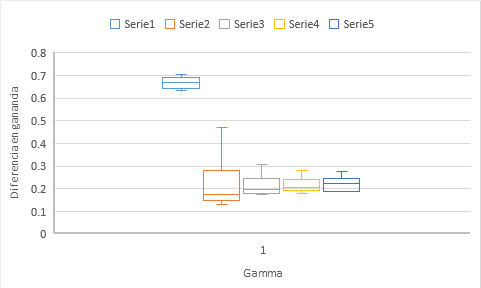
\includegraphics[scale=1]{Cajas1.png}
	\caption{Diagramas BoxPlot para la variable Gamma}
	\label{Cajas1}
\end{figure}

\begin{figure} [H]
	\centering
	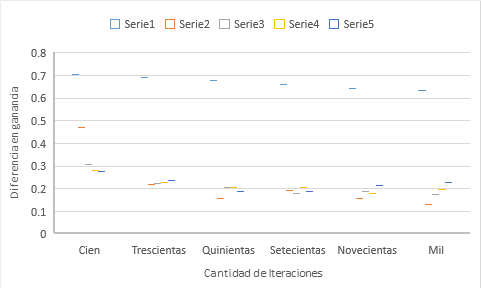
\includegraphics[scale=1]{Cajas1_1.png}
	\caption{Diagramas BoxPlot para la variable Iteraciones}
	\label{Cajas1_1}
\end{figure}

Para corroborar esta observación se genera el análisis de varianza ANOVA para los datos de la misma tabla \ref{exp0}, cuyo resultado se presenta en la tabla \ref{tab:Anova1}. 

\begin{table}[H]
\centering\caption{ANOVA para Distancias en ganancias usando Gamma}
\small
\begin{tabular}{lrrrr} \\ 
%\multicolumn{5}{c}{\textbf{ANÁLISIS DE VARIANZA}}             \\
\multicolumn{1}{c}{\textit{\textbf{\begin{tabular}[c]{@{}c@{}}Origen de las \\ \\ variaciones\end{tabular}}}} & \multicolumn{1}{c}{\textit{\textbf{\begin{tabular}[c]{@{}c@{}}Promedio de \\ \\ los cuadrados\end{tabular}}}} & \multicolumn{1}{c}{\textit{\textbf{F}}} & \multicolumn{1}{c}{\textit{\textbf{Probabilidad}}} & \multicolumn{1}{c}{\textit{\textbf{\begin{tabular}[c]{@{}c@{}}Valor crítico \\ \\ para F\end{tabular}}}} \\ \hline
                  & \multicolumn{1}{l}{}                                               & \multicolumn{1}{l}{}                    & \multicolumn{1}{l}{}                               & \multicolumn{1}{l}{}                                          \\
\textbf{Gamma}                                                                                                & 0.244513                                    & 118.074                              & 1.297E-13                                       & 2.86608                                        \\ 
\textbf{Iteraciones}                                                                                             & 0.013214                                       & 6.381                            & 0.00107                                       & 2.71089         \\ \hline                            
\end{tabular}
\label{tab:Anova1}
\end{table}

Para la primera variable, $Gamma$, se obtiene el valor de \textit{F} mayor al de \textit{F crítica} y una probabilidad muy baja $(P<0.05)$, lo que indica que existe una diferencia significativa en Gamma que afecta la variable dependiente.

Para la segunda variable, $Iteraciones$, se obtiene el valor de \textit{F} mayor al de \textit{F crítica} y una probabilidad baja $(P<0.05)$, lo que indica que también existe una diferencia significativa en el número de iteraciones que afecta la variable dependiente, pero no de la misma forma que la variable $Gamma$, tal como se había planteado al analizar las gráficas BoxPlot.

Se quiere entonces, encontrar un valor de Gamma que ofrezca buenos resultados, y estimar hasta donde la cantidad de iteraciones puede disminuir considerablemente el valor de la variable dependiente, que corresponde a la diferencia entre las ganancias obtenidas y la ganancia real, para lo que se plantean los experimentos siguientes.

\subsubsection{Experimento dos}

%Se diseña un experimento con dos variables independientes: T y $\gamma$, correspondientes a la cantidad de iteraciones y a la variable que, multiplicada por la ganancia total asociada a la secuencia de nodos que se haya probado, como parámetro de aprendizaje. Se recuerda que la variable dependiente corresponde a la diferencia normalizada de las ganancias y que también se calcula el porcentaje de veces que el vector final corresponde al esperado cuyo valor debe estar cercano al 100\%, cuando el de la diferencia de ganancia se acerque al 0\%.

 Para este experimento se usan valores para T de 100, 1000, 10000 y 100000 iteraciones y valores de $\gamma$ de $10^{0}$, $10^{-1}$, $10^{-2}$, $10^{-3}$, $10^{-4}$, $10^{-5}$, $10^{-6}$. Al ejecutar este experimento varias veces, se encuentra que los valores de sus resultados para los mismo valores de T y de $\gamma$, tienen tendencias marcadas, lo que permite establecer que la influencia de la aleatoriedad en estos resultados es menor que la que se observó en los experimentos anteriores. 

\begin{table}[H]
\caption{Experimento tres}
\centering
\begin{tabular}[c]{llll}
\multicolumn{1}{p{2.9cm}}{\textbf{GRÁFICA PARA $\gamma$}} & \multicolumn{1}{p{2.9cm}}{\textbf{GRÁFICA PARA $T$}} & \multicolumn{1}{p{2.9cm}}{\textbf{GRÁFICA PARA $T$ y $\gamma$}} & \multicolumn{1}{p{2.9cm}}{\textbf{ANOVA}}  \\ \hline
\multicolumn{1}{|l|}{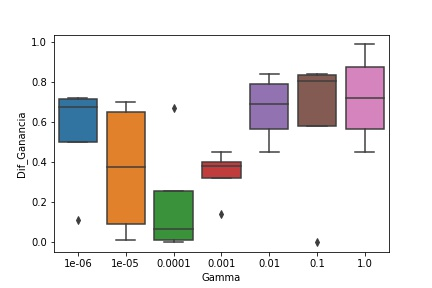
\includegraphics[align=t, width=33mm]{cajasGamma_exp31.jpg}}    & \multicolumn{1}{l|}{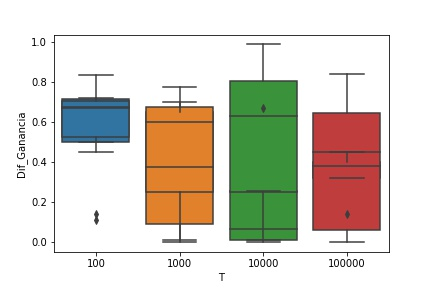
\includegraphics[align=t, width=33mm]{cajasT_exp31.jpg} } & \multicolumn{1}{l|}{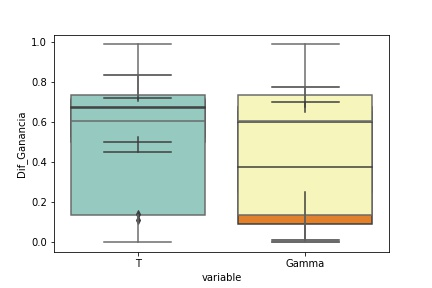
\includegraphics[align=t, width=33mm]{cajasT_Gamma_exp31.jpg} } &
\multicolumn{1}{p{3cm}|}{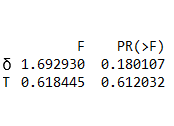
\includegraphics[align=t, width=30mm]{Anova31.png}}     \\ \hline
\multicolumn{1}{|l|}{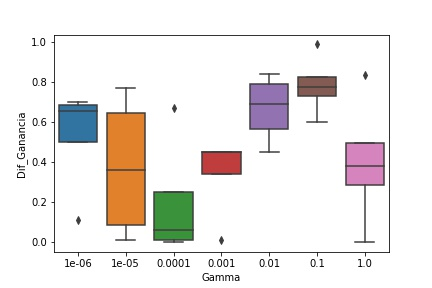
\includegraphics[align=t, width=33mm]{cajasGamma_exp32.jpg}}    & \multicolumn{1}{l|}{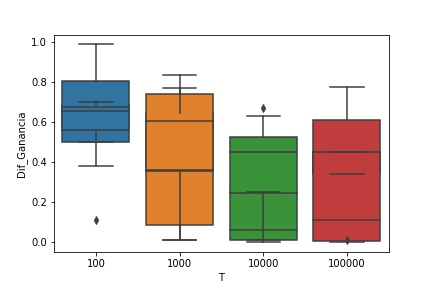
\includegraphics[align=t, width=33mm]{cajasT_exp32.jpg} } & \multicolumn{1}{l|}{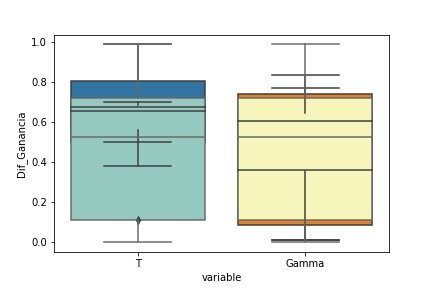
\includegraphics[align=t, width=33mm]{cajasT_Gamma_exp32.jpg} } & \multicolumn{1}{p{3cm}|}{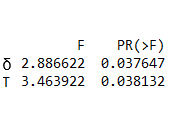
\includegraphics[align=t, width=30mm]{Anova32.png}} \\ \hline
\multicolumn{1}{|l|}{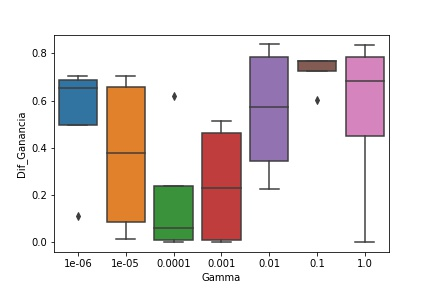
\includegraphics[align=t, width=33mm]{cajasGamma_exp33.jpg}}    & \multicolumn{1}{l|}{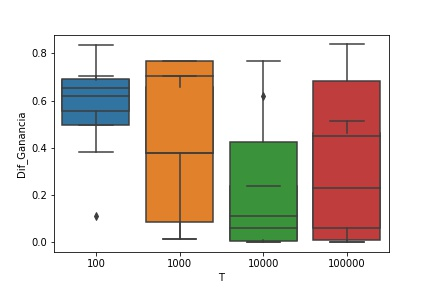
\includegraphics[align=t, width=33mm]{cajasT_exp33.jpg} } & \multicolumn{1}{l|}{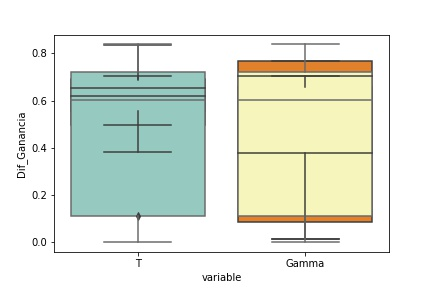
\includegraphics[align=t, width=33mm]{cajasT_Gamma_exp33.jpg} } & \multicolumn{1}{p{3cm}|}{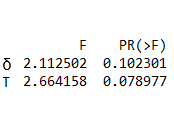
\includegraphics[align=t, width=30mm]{Anova33.png}} \\ \hline
\end{tabular}
\label{exp3}
\end{table}

Tres de estos resultados se pueden ver en la tabla \ref{exp3}, donde, aunque el valor del estadístico de prueba F de las tablas ANOVA aún no presenta valores lejanos a la unidad, el ejemplo de la segunda fila muestra valores para $PR(>F)$ menores a 0.05, para ambas variables. 
 
Estos cambios, que se ocasionan por la influencia de la aleatoriedad que aún se presenta, no permiten, una vez más, concluir que los valores de alguna de estas variables independientes influye efectivamente en los de la variable dependiente. 
 
Aún así, en las gráficas de la tabla \ref{exp3} se observa que se obtienen resultados de la diferencia normalizada de ganancias con medias que están por debajo del 80\% y que llegan a tomar valores cercanos al 0\%, especialmente con los valores más altos de la variable $T$ y más bajos para la variable $\gamma$. Lo anterior sugiere que con pequeños pasos y mayor cantidad de ellos, se puede llegar a obtener mejores resultados, lo que se verifica en el siguiente experimento.

\subsubsection{Experimento tres}

%Se diseña un experimento con las dos variables independientes: T y $\gamma$, correspondientes a la cantidad de iteraciones y a la variable que, multiplicada por la ganancia total asociada a la secuencia de nodos que se haya probado, como parámetro de aprendizaje. Se maneja la misma variable dependiente, corresponde a la diferencia normalizada de las ganancias como en los experimentos previos.

Para este experimento se usan valores para T de 10000 a 100000 iteraciones con intervalos de 10000 y valores de $\gamma$ del orden de $10^{-4}$, teniendo en cuenta que fue la cifra que mostró los valores más bajos para la variable dependiente. 

Las gráficas correspondientes a tres ejecuciones de este experimento con sus gráficas y resultados del ANOVA, se presentan en la tabla \ref{exp4}.

\begin{table}[]
\caption{Experimento cuatro}
\centering
\begin{tabular}[c]{llll}
\multicolumn{1}{p{2.95cm}}{\textbf{GRÁFICA PARA $\gamma$}} & \multicolumn{1}{p{2.95cm}}{\textbf{GRÁFICA PARA $T$}} & \multicolumn{1}{p{2.95cm}}{\textbf{GRÁFICA PARA $T$ y $\gamma$}} & \multicolumn{1}{p{2.95cm}}{\textbf{ANOVA}}  \\ \hline
\multicolumn{1}{|l|}{\includegraphics[align=t, width=33mm]{cajasGamma_exp4.jpg}}    & \multicolumn{1}{l|}{\includegraphics[align=t, width=33mm]{cajasT_exp4.jpg} } & \multicolumn{1}{l|}{\includegraphics[align=t, width=33mm]{cajasT_Gamma_exp4.jpg} } &
\multicolumn{1}{p{3.2cm}|}{\includegraphics[align=t, width=30mm]{Anova4.png}}     \\ \hline
\multicolumn{1}{|l|}{\includegraphics[align=t, width=33mm]{cajasGamma_exp42.jpg}}    & \multicolumn{1}{l|}{\includegraphics[align=t, width=33mm]{cajasT_exp42.jpg} } & \multicolumn{1}{l|}{\includegraphics[align=t, width=33mm]{cajasT_Gamma_exp42.jpg} } & \multicolumn{1}{p{3.2cm}|}{\includegraphics[align=t, width=30mm]{Anova42.png}} \\ \hline
\multicolumn{1}{|l|}{\includegraphics[align=t, width=33mm]{cajasGamma_exp43.jpg}}    & \multicolumn{1}{l|}{\includegraphics[align=t, width=33mm]{cajasT_exp43.jpg} } & \multicolumn{1}{l|}{\includegraphics[align=t, width=33mm]{cajasT_Gamma_exp43.jpg} } & \multicolumn{1}{p{3.2cm}|}{\includegraphics[align=t, width=30mm]{Anova43.png}} \\ \hline
\end{tabular}
\label{exp4}
\end{table}

Aunque las gráficas generadas al ejecutar este experimento varias veces, con los mismo valores de T y de $\gamma$, parecen diferentes, mantienen valores para la variable independiente muy cercanos a cero, con valores inferiores al 2\% para todos los casos probados, lo que permite establecer una baja influencia de la aleatoriedad.

Los  valores del estadístico de prueba $F$ y de $PR(>F)$ de las tablas ANOVA muestran que no hay una dependencia entre los valores de la variable $\gamma$ y los resultados de la variable dependiente, puesto que $F$ toma valores cercanos a 1 y, $PR(>F)$ es mayor a 0.05. 

La independencia aparente de la variable $\gamma$ en los valores que toma la diferencia promedio de ganancias resulta ser un aspecto deseable para el experimento, puesto que los dos valores tomados para $Gamma$ solo difieren en $1*10^{-5}$, como se aprecia más claramente en la figura \ref{CajasGamma} así que lo ideal era obtener resultados similares. 

\begin{figure}[H]
	\centering
	\includegraphics[scale=0.5]{cajasGamma_exp4.jpg}
	\caption{Diferencia normalizada de ganancias para $T$ y $\gamma$}
	\label{CajasGamma}
\end{figure}

De otra parte, en dos de los tres casos hay influencia de los valores que se dan a la variable $T$ sobre los obtenidos en la variable dependiente, ya que el valor de la probabilidad $PR(>F)$ es menor que 0.05; aspecto que resulta positivo para el modelo, porque se acercan a un control inicial de los efectos de la aleatoriedad.

De aquí que, con cualquier valor de T superior a 50000 iteraciones se obtuvieron excelentes resultados, con medias en la diferencias promedio de ganancias inferiores a 0.003 y varianzas muy pequeñas. Se elige entonces el valor de 100000 para la variable T y de $10^{-4}$ para la variable $\gamma$, para generar el histograma en los que se apreciará cómo, efectivamente, la mayor parte de los valores de la variable dependiente se acerca a cero. Dicho histograma se muestra en la figura \ref{histo4}.

\begin{figure}[H]
	\centering
	\includegraphics[scale=0.5]{Histograma_gamma3.jpg}
	\caption{Diferencia normalizada a la ganancia real}
	\label{histo4}
\end{figure}

Vale aclarar que esta ejecución se realizó varias veces, encontrando siempre resultados similares, por lo que no se hace ningún comparativo adicional, sino que  se concluye que los valores probados en este experimento arrojarán el resultado correcto.

Teniendo establecidos los parámetros de número de iteraciones y del factor de aprendizaje $\delta$, se procede a probar el desempeño del algoritmo con grafos generados por él mismo.

\section{Generando el grafo aleatoriamente}

Se ejecutó el programa de forma que permitiera como datos de entrada, además de los ya implementados, la cantidad de etapas del grafo y la cantidad de nodos en cada etapa. La matriz de adyacencia se ha programado para que cada nodo tenga al menos uno adyacente de la siguiente etapa, excepto si es de la ultima etapa, además para que la densidad de conectividad entre los nodos sea del 66.67\%. 

Los valores de los \texit{bandits} se generan también de forma aleatoria con media en cero y desviación estándar de una unidad, pero se modifican computacionalmente para que uno de los nodos de cada etapa, elegido al azar, tenga asociada una ganancia positiva superior a la de los demás nodos de su etapa. Además, se ajustaron estos valores para que las ganancias sean del orden de las centenas, como los del grafo para el que se habían ajustado los parámetros de cantidad de iteraciones y de $\delta$, ya que este último depende de la magnitud de la ganancia que se obtenga en cada iteración.

El programa arroja resultados favorables con una cantidad de etapas $L$ entre 5 y 12, observados en la convergencia de sus ganancias hacia la mayor ganancia real dentro de los caminos probados por el algoritmo, como la que se aprecia en la figura \ref{Gangraforandom}. Uno de los casos se verifica manualmente, obteniendo el grafo a partir de la matriz de adyacencia generada aleatoriamente y de los valores generados para sus \texit{bandits}, con un valor de $L$ de 9 etapas y los siguientes valores para la cantidad de nodos por etapa: [1. 3. 4. 4. 3. 1.].

La gráfica se muestra en la figura \ref{graforandom} y su matriz de adyacencia es la siguiente:

\renewcommand{\arraystretch}{0.5}
%\begin{equation}
A = 
$\begin{bmatrix}
%\hspace{2cm}

0, 0, 1, 1,  0,  0,  0,  0,  0,  0,  0, 0, 0, 0, 0, 0\\
0, 0, 0, 0,  1,  1,  1,  0,  0,  0,  0, 0, 0, 0, 0, 0\\
0, 0, 0, 0,  0,  1,  0,  0,  0,  0,  0, 0, 0, 0, 0, 0\\
0, 0, 0, 0,  1,  0,  1,  1,  0,  0,  0, 0, 0, 0, 0, 0\\
0, 0, 0, 0,  0,  0,  0,  0,  1,  1,  1, 0, 0, 0, 0, 0\\
0, 0, 0, 0,  0,  0,  0,  0,  0,  0,  1, 1, 0, 0, 0, 0\\
0, 0, 0, 0,  0,  0,  0,  0,  1,  1,  0, 1, 0, 0, 0, 0\\
0, 0, 0, 0,  0,  0,  0,  0,  0,  1,  1, 0, 0, 0, 0, 0\\
0, 0, 0, 0,  0,  0,  0,  0,  0,  0,  0, 0, 1, 0, 1, 0\\
0, 0, 0, 0,  0,  0,  0,  0,  0,  0,  0, 0, 0, 1, 0, 0\\
0, 0, 0, 0,  0,  0,  0,  0,  0,  0,  0, 0, 1, 1, 1, 0\\
0, 0, 0, 0,  0,  0,  0,  0,  0,  0,  0, 0, 1, 1, 1, 0\\
0, 0, 0, 0,  0,  0,  0,  0,  0,  0,  0, 0, 0, 0, 0, 1\\
0, 0, 0, 0,  0,  0,  0,  0,  0,  0,  0, 0, 0, 0, 0, 1\\
0, 0, 0, 0,  0,  0,  0,  0,  0,  0,  0, 0, 0, 0, 0, 1\\
0, 0, 0, 0,  0,  0,  0,  0,  0,  0,  0, 0, 0, 0, 0, 0
\end{bmatrix}$

Así mismo el vector de \textit{bandits} generado de forma aleatoria fue el siguiente:

$B$ = [196.02255721, 9.32455363, 47.72564534, 66.21935444, 275.7996602, 6.62172573, 190.49629308, 13.33418851, 210.36419278, 37.39029137, 191.40773576, 117.1717095, 40.02228911, 220.45436046, 32.32878409, -125.16559689]

\begin{figure}[H]
	\centering
	\includegraphics[scale=0.4]{GrafoRandom.png}
	\caption{Grafo generado en forma aleatoria}
	\label{graforandom}
\end{figure}

\subsection{Prueba}

Se recuerda que las variables independientes son: la cantidad de Iteraciones y el factor de aprendizaje $deltha$. Se recuerda también que este último parámetro se obtuvo de multiplicar el coeficiente $Gamma$ por la ganancia que cada vector solución va recibiendo al final de la iteración en que se genera. El valor asignado al parámetro de $T$ es de 80000 iteraciones y el de $\gamma$ es de 0.000003. 

De otra parte, la variable dependiente que se ha manejado en los experimentos anteriores ha sido el promedio de diferencias normalizadas entre las ganancias obtenidas y la ganancia óptima, pero para probar el modelo con el grafo aleatorio, se adicionó un indicador de salida que cuenta las veces que el vector solución generado por la aplicación correspondió con el vector óptimo.

Los valores óptimos del vector solución y de su ganancia real asociada los establecen la misma aplicación, guardando el valor de la ganancia real máxima que se vaya obteniendo y su argumento (es decir el vector objeto de dicha ganancia), puesto que, con la gran cantidad posible de rutas en un grafo aleatorio, sería tedioso conseguir estos valores manualmente.

Luego de la 80000 iteraciones con los parámetros ya explicados se obtuvieron las siguientes salidas:

\begin{itemize}
\item Promedio de la diferencia entre las ganancias obtenidas en cada iteración y la ganancia óptima: 0.019839554951030753, que es un valor inferior al 2\%.
\item Porcentaje de aciertos entre los vectores generados en cada iteración y el vector óptimo: 0.9531375, valor que supera el 95\% de coincidencias.
\item Vector óptimo = [0, 3, 4, 10, 13, 15]
\end{itemize}

Revisado el grafo de forma manual, se observa que el vector encontrado corresponde con el real, como se puede corroborar en la figura \ref{graforandom}.

Además se generó la gráfica de convergencia de la ganancia que se obtienen en cada iteración y el resultado obtenido se muestra en la figura \ref{Gangraforandom}.

\begin{figure}[]
	\centering
	\includegraphics[scale=0.8]{GanGrafoRandom.png}
	\caption{Convergencia de ganancia con un grafo generado en forma aleatoria}
	\label{Gangraforandom}
\end{figure}

En esta figura el eje horizontal corresponde al número de la iteración y el eje vertical a la ganancia obtenida en cada iteración. 

Es importante aclarar que, no se espera que el promedio de diferencias entre ganancias llegue a ser cero ni que el porcentaje de aciertos del vector generado con el vector óptimo llegue a ser uno, puesto que el autómata toma un tiempo en aprender la ruta óptima y los valores que haya tenido que probar para este aprendizaje, siempre se tendrán en cuenta para el cálculo de estos valores. 

Finalmente se resalta el hecho de que la gráfica se estabiliza después de solo 10000 iteraciones, pero es necesario ejecutar cerca de 100000 para obtener resultados aceptable en el promedio normalizado de diferencias entre ganancias y en el porcentaje de aciertos con el vector óptimo; conseguir un criterio de parada para el algoritmo que disminuya el número de iteraciones será parte de la continuidad de esta investigación.